\documentclass[12pt]{article}
\usepackage{graphicx}
\usepackage{amsfonts}
\usepackage{amssymb}
\usepackage{mathrsfs}
\usepackage{amsmath}
\usepackage{subfig}
\usepackage{algorithm2e}

\SetKwInOut{Parameter}{parameter}

\usepackage{enumitem}
\textheight 225mm
\textwidth 166mm
\oddsidemargin 0mm
\evensidemargin 0mm
\topmargin -14mm
\parindent 20pt
\pagestyle{plain}
\pagenumbering{arabic}
\renewcommand{\baselinestretch}{1.18}

\usepackage[unicode]{hyperref}
%\usepackage[numbers,sort&compress]{natbib}
\usepackage{booktabs}
% With this package you can set the size of the margins manually:
\usepackage[margin=1in]{geometry}
\usepackage{amssymb}

%\newenvironment{claim}[1]{\par\noindent\underline{Claim:}\space#1}{}
%\newenvironment{claimproof}[1]{\par\noindent\underline{Proof:}\space#1}{\hfill $\blacksquare$}
\usepackage[hyperref,amsmath, thmmarks]{ntheorem}
\usepackage{mathtools}
\DeclarePairedDelimiter\ceil{\lceil}{\rceil}
\DeclarePairedDelimiter\floor{\lfloor}{\rfloor}

\newtheorem{claim}{Claim}
\theoremsymbol{\rule{1ex}{1ex}}
\newtheorem{proof}{Proof}
\theoremsymbol{\rule{1ex}{1ex}}
\newtheorem{claimproof}{Proof of claim}
\title{Traverse Points}

\author{Yuhao Zhang}

\date{\today}
\begin{document}
\maketitle
% Enter the exercise number, your name and date here:
%\noindent\parbox{\linewidth}{
% \parbox{.25\linewidth}{ \large HW2 }\hfill
% \parbox{.5\linewidth}{\begin{center} \large Yuhao Zhang \end{center}}\hfill
% \parbox{.2\linewidth}{\begin{flushright} \large Jan 22, 2018 \end{flushright}}
%}
%\noindent\rule{\linewidth}{2pt}


%\section{Introduction}
%
%Briefly introduce the problem here. Describe what you have to do and what the goal is. Make sure to cite any references that you might use \cite{knuth}.
\section{Introduction}
This project is a model of the car-like robot and a control algorithm to traverse several waypoints with specific coordinates and poses. The code is for Sunfounder's PiCar-V platform and no sensors are involved: the car receives no feedback from its motion and surroundings.
\section{Kinematics and control law}
\label{kine}
Ackerman model can be used to describe the kinematics of a car-like robot: 
$$\frac{d x}{dt}=v\cos \theta,$$
$$\frac{d y}{dt}=v\cos \theta,$$
$$\frac{d \theta}{dt}=\frac{v}{L}\tan \gamma,$$
where $(x,y)$ is the position of the middle point of the back wheel axis of the robot in world reference frame. $\theta$ is the angle of pose of the robot. The steering wheel angle is $\gamma$ and the velocity of the back wheel is $v$. $L$ is the length of the vehicle or wheel base.

These equations can be re-written as:
$$
\begin{pmatrix}
\frac{d x}{dt} \\
\frac{d \omega}{dt} \\
\frac{d \theta}{dt} \\
\end{pmatrix}
=
\begin{pmatrix}
\cos \theta & 0 \\
\sin \theta & 0 \\
0 & 1\\
\end{pmatrix}
\begin{pmatrix}
v \\
\omega
\end{pmatrix}.
$$
With the initial position-pose $(x,y,\theta)$ and the goal $(x^*,y^*,\theta^*)$, it is more convenient to write the equations in polar system via a transformation:
$$\rho=\sqrt{\Delta_x^2+\Delta_y^2},$$
$$\alpha=\arctan \frac{\Delta_y}{\Delta_x}-\theta,$$
$$\beta=-\theta-\alpha+\theta^*.$$

The linear control law for $-\pi/2<\alpha\le \pi/2$, i.e. the waypoint is in front of the vehicle is:
$$v=k_\rho \rho,$$
$$\omega=k_\alpha \alpha+k_\beta \beta,$$
where $k_\rho$, $k_\alpha$, $k_\beta$ are arbitrary coefficients that satisfies $k_\rho>0, k_\beta<0,k_\alpha-k_\rho>0.$

The control law for the cases where the waypoint is behind the vehicle is the same as above, but with transformed angles:

$$\alpha'=-\pi-\beta,$$
$$\beta'=-\pi-\alpha,$$
and $v'=-v$.

\section{Pose estimation}
\label{pose}
Without the feedback from sensors, it is required to estimate the motion from the kinematics of the robot directly. Using the linear approximation of the kinematics equations for a short time period $\Delta t$ one can obtain
$$\Delta(x,y,\theta)=(v\cos \theta \Delta t ,v \sin \theta \Delta t, v/L \tan \gamma \Delta t).$$

Alternatively, the exact solution can be obtained by solving these differential equations directly:
$$\Delta(x,y,\theta)=(R_b\sin(K\Delta t),R_b(1-\cos(K\Delta t)),K\Delta t),$$
where $R_b=L/\tan \gamma$ and $K=v/R_b$. However, this estimation is non-linear and makes the control law purposed unstable. Therefore the linear approximation will be used in the following sections.


\section{Control algorithm implementation}
The control law purposed in Sec.(\ref{kine}) and the pose estimation algorithm purposed in Sec.(\ref{pose}) have been implemented in \texttt{drive\_to\_points.ipynb}.  Given the input \texttt{waypoints.txt}, the generated trajectory and the estimated poses along it is plotted as Fig.()
\begin{figure}[htbp]
\centering
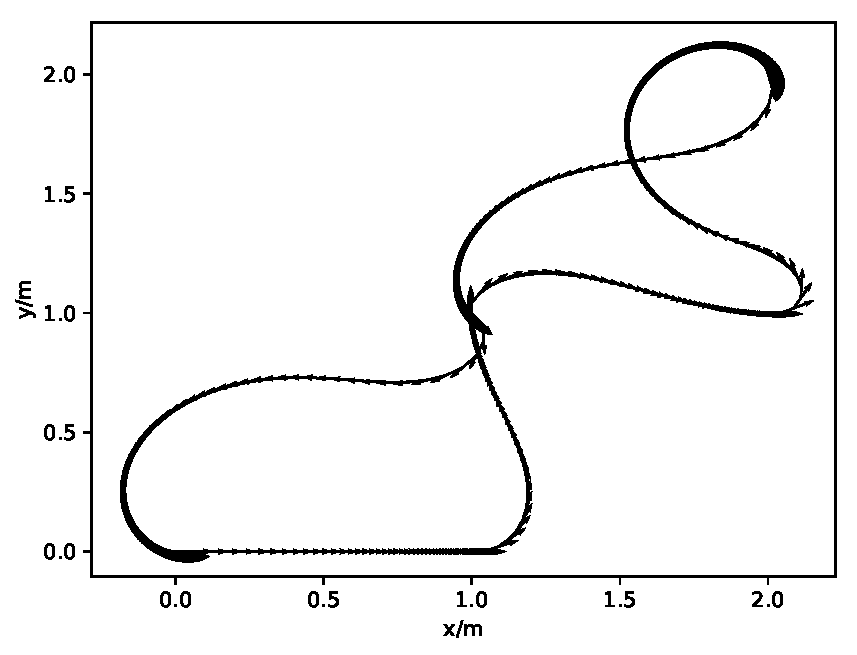
\includegraphics[width=0.5\textwidth]{../ideal_traj.pdf}
\caption{1000 different 100$\times$100 lattices with different $p$ values, the shortest path and the life time of fire}\label{fig3}
\end{figure}

\begin{enumerate}[label=(\alph*)]
\item Beginning with Brown corpus and removing the stop-words and punctuation, making everything lowercase.
\item Selecting the most commonly used words in the corpus. $V: \text{most commonly used 5000 words}$ and $C: \text{most commonly used 1000 words}$.
\item For each word $w \in V$ and denote context $B_w^k$: in a text stream, for a word $w$, we denote the surrounding $2k$ words of every occurrence of $w$ as its context, with $k$ words before it and $k$ words after it. 
\item Define $Pr(c|w)$ as given $w \in V$, the probability that $c \in C$ and $c \in B_w^k$.
\item Then calculate $$\Phi_c(w)= max(0,\log \frac{Pr(c|w)}{Pr(c)})$$
for each $w$.
\item Apply PCA to $\Phi_c(w)$, to acquire a 100-dimensional representation of $\Phi_c(w)$, denoted as $\Psi(w)$
\end{enumerate}

\section{Nearest neighbor test}
The result of nearest neighbor search for a random collection of 25 words and the corresponding cosine similarity is listed in Tab.(\ref{tab1}).
There are pairs such as \textit {proceedings, midst}, easy to correspond to sentences like \textit {...in the midst of proceedings...}. And pairs such as \textit {external, internal}, \textit {letter, book}, \textit {day, week} and \textit {gray, green}, which are words in the same domain. There are also confusing pairs such as \textit {jail, di}. What is more, it also shows some worrying result like \textit {customers, drugs}
\begin{table}[!h]
\centering
\caption{Experiment results for nearest neighbor}
\label{tab1}
\begin{tabular}{llr}

$w$    & $c$ & Cosine similarity  \\
\hline
external        &internal        &0.463563\\
committed      & straightened  &  0.228246\\
disposal     &   specialists    & 0.252870\\
commission  &    department    &  0.473976\\
chair       &    knees     &      0.473293\\
torn        &    lap         &    0.197125\\
judges       &   stem         &   0.214150\\
joe         &    cousin     &     0.460737\\
proceedings    & midst      &     0.053407\\
customers   &    drugs      &     0.344528\\
proved     &     examine       &  0.597234\\
poverty    &     midst        &   0.197982\\
letter       &   book         &   0.446783\\
construction   & plant    &       0.502133\\
identify     &   adding    &      0.306849\\
day        &     week       &     0.302847\\
gray        &    green    &       0.212985\\
varied  &        shared     &     0.442941\\
drank    &       hay      &       0.191549\\
drawn    &       gray      &      0.506984\\
package    &     hay        &     0.286869\\
jail        &    di         &     0.234771\\
convenience  &   hay      &       0.212920\\
taxes      &     estimated      & 0.327287\\
bars        &    puts     &       0.251591\\
\hline
\end{tabular}
\end{table}



\section{Clustering}
Next $V$ is clustered into 100 groups based on there embeddings via \texttt{sklearn.cluster}. Some of the top clusters are shown below:

A cluster commonly used for weather report:

\texttt{summer spring start winter spent coming sun fall suddenly afternoon
saturday instead evening hot sunday started hours opened late cold}

A cluster describing international affairs and education:

\texttt{aid vocational support assistance financial planning services technical defense schools
programs training private international research act foreign community medical provide}

A cluster talking about production economy:

\texttt{income estimated net capital annual operating additional average pay property
increased farm rates billion price amount stock increase production pressure}

And a cluster about military:

\texttt{staff division army corps activities personnel management facilities services forces
association peace research medical committee department force industrial military service}
%\begin{figure}[htbp]
%\centering
%\includegraphics[width=0.5\textwidth]{./src/lctwomethods.eps}
%\caption{Learning curve for steepest-direction coordinate descent and random-feature coordinate descent.}\label{fig1}
%\end{figure}

%\begin{table}[hp]
%\centering
%\caption{Experiment results}
%\label{tab1}
%\begin{tabular}{llr}
%
%$M$    & Prototype & Error rate (\%) \\
%\hline
%1000      & random    & $13.02 \pm  0.73$    \\
%          & random*        & $11. 84 \pm 0.20$      \\
%5000       & random     & $6.63 \pm 0.11$      \\
%		& random*     &$6.42 \pm 0.22$      \\
%10000       & random     & $5.07 \pm 0.2$     \\
%		 & random*      & $4.8 \pm 0.26$       \\
%\hline
%\end{tabular}
%\end{table}







%\subsection{Task 3}
%For 1000 different 100$\times$100 lattices with different $p$ values, the shortest path and the life time of fire is plotted in Fig.(\ref{fig3}). It can be seen clearly that the curves have a phase change point at $p_c\approx0.59$, after which the minimal step and life of fire drop quickly and approximates 100, the width of lattice.
%
%\begin{figure}[htbp]
%\centering
%\includegraphics[width=0.5\textwidth]{../figures/N100pvariable.eps}
%\caption{1000 different 100$\times$100 lattices with different $p$ values, the shortest path and the life time of fire}\label{fig3}
%\end{figure}
%
%For different values of width of lattice $N$, we use 1000 different random lattices per $N$ to find the correlation between the ratio of spanning cluster and the $p$ value, which is plotted in Fig.(\ref{fig4})
%
%
%\begin{figure}[htbp]
%\centering
%\includegraphics[width=0.5\textwidth]{../figures/ratio.eps}
%\caption{1000 different lattices of $N=50, 100, 200$ with different $p$ values, the ratio of the spanning cluster}\label{fig4}
%\end{figure}
%
%
%\section{Discussion}
%It can be found through these figures that $p_c\approx0.59$ and it is irrelevant to the width of lattice $N$.
%\begin{thebibliography}{99}
%
%\bibitem{knuth}
%  Knuth, Ervin D.,
%  \emph{The art of computer programming}, 
%  Addison Wesley, Massachusetts,
%  3rd edition,
%  1997.
%
%\end{thebibliography}

\end{document}